\chapter{Các đại lượng quan sát giao hoán, pha năng lượng và sự tiến động của spin}

\lectureoverview{Chúng ta bắt đầu với ý nghĩa định tính của độ bất định. Hai đại lượng quan sát chỉ có thể đồng thời xác định khi chúng có một cơ sở riêng chung đầy đủ, và điều này tương đương với việc các toán tử của chúng giao hoán. Sau đó ta ôn lại sự tiến hóa unita và phương trình Schr\"odinger, so sánh các giao hoán tử với các ngoặc Poisson cổ điển, giải phương trình phụ thuộc thời gian trong cơ sở năng lượng, và áp dụng kết quả cho một spin trong từ trường. Phép tính cuối cùng cho ta sự tiến động của các giá trị kỳ vọng của spin, hai mức năng lượng của một Hamiltonian spin tổng quát, và sự phân biệt giữa một giá trị kỳ vọng theo phương ngang với một photon có năng lượng bằng một nửa độ chênh năng lượng.}

Hệ spin hai trạng thái vẫn là hệ lượng tử đơn giản nhất của chúng ta. Một không gian Hilbert ba trạng thái sẽ là khả năng trừu tượng đơn giản kế tiếp; hai spin thì đã có bốn trạng thái cơ sở trực giao. Ta sẽ chưa ghép hai spin lại, mặc dù bước đó đã ở rất gần và sẽ kéo theo đan rối. Trước hết, ta nên hoàn tất bài toán một spin và đặt các ý tưởng về độ bất định và sự tiến hóa theo thời gian trên nền tảng vững chắc hơn.

\section{Khi nào hai đại lượng có thể đồng thời xác định}

Một phép đo tốt là phép đo lặp lại được. Nếu đo một đại lượng quan sát và thu được giá trị \(l\), thì phép đo lặp lại ngay sau đó phải cho lại chính giá trị ấy. Vì vậy, phép đo thứ nhất phải để hệ, ít nhất là trong chốc lát, ở một trạng thái riêng của toán tử tương ứng:
\begin{equation}
L\ket{l}=l\ket{l}.
\end{equation}
Phát biểu mang tính thao tác này là đủ để làm lộ ra nguồn gốc định tính của độ bất định.

Giả sử hai đại lượng quan sát \(L\) và \(M\) có thể được đo đồng thời. Một phép đo đồng thời phải khiến cả hai giá trị được báo cáo đều xác định. Vì thế, các trạng thái có thể có sau phép đo của nó phải là các vectơ riêng đồng thời của cả hai toán tử. Trong khuôn khổ hữu hạn chiều dùng ở đây, ta có thể chọn một tập trực chuẩn đầy đủ \(\{\ket{i}\}\) thỏa mãn
\begin{equation}
L\ket{i}=l_i\ket{i},
\qquad
M\ket{i}=m_i\ket{i}.
\label{eq:l5-common-eigenvectors}
\end{equation}

\begin{remark}
Từ \emph{cơ sở} ở đây sẽ được hiểu là một cơ sở trực chuẩn đầy đủ. Đại số tuyến tính cho phép các cơ sở không trực giao, nhưng quy ước trực chuẩn đặc biệt tự nhiên đối với các trạng thái lượng tử. Các trị riêng suy biến để lại tự do bên trong một không gian riêng; trong không gian đó, các vectơ riêng có thể được chọn trực chuẩn.
\end{remark}

\begin{theorem}
Hai đại lượng quan sát Hermite hữu hạn chiều đo được đồng thời khi và chỉ khi chúng có một cơ sở riêng chung đầy đủ; tương đương, khi chúng giao hoán.
\end{theorem}

Chiều thuận suy ra ngay từ Phương trình~\eqref{eq:l5-common-eigenvectors}. Tác dụng theo một thứ tự cho
\begin{align}
ML\ket{i}
&=M\bigl(l_i\ket{i}\bigr)\\
&=l_i m_i\ket{i},
\end{align}
trong khi thứ tự ngược lại cho
\begin{align}
LM\ket{i}
&=L\bigl(m_i\ket{i}\bigr)\\
&=m_i l_i\ket{i}.
\end{align}
Các trị riêng là những số thông thường, nên \(l_i m_i=m_i l_i\). Vì vậy \(ML\) và \(LM\) tác dụng giống hệt nhau lên mọi phần tử của một cơ sở và do đó lên mọi trạng thái:
\begin{equation}
[L,M]\equiv LM-ML=0.
\label{eq:l5-commuting-condition}
\end{equation}

\begin{figure}[htbp]
\centering
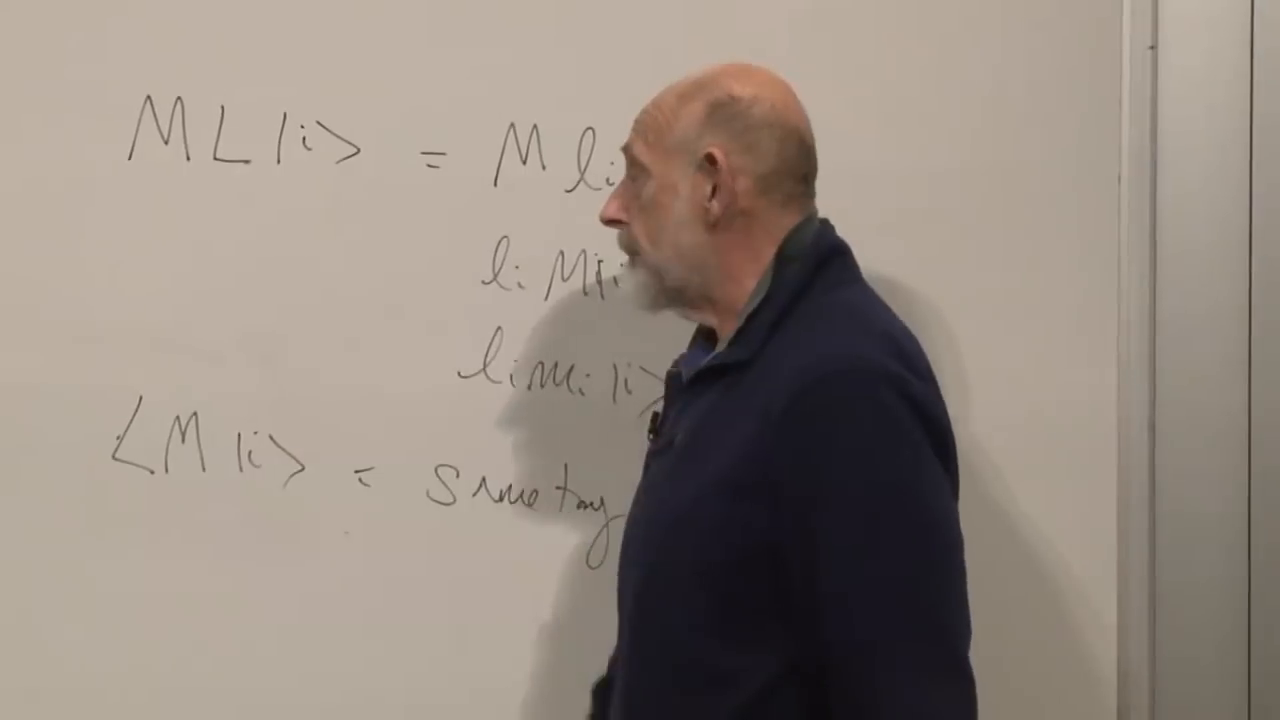
\includegraphics[width=0.86\textwidth]{lecture_05_figure_02.png}
\caption{Lập luận bằng vectơ riêng chung dẫn đến \(LM-ML=[L,M]=0\).}
\lectureframe{00:10:30}
\end{figure}

Mệnh đề đảo cũng đúng: các toán tử Hermite giao hoán có thể được chéo hóa đồng thời. Nếu một toán tử có một không gian riêng suy biến, thì toán tử kia bảo toàn không gian riêng đó, và có thể được chéo hóa bên trong nó. Lặp lại việc này trong mọi không gian riêng sẽ tạo ra một cơ sở riêng chung đầy đủ.

Các toán tử Pauli cho phản ví dụ quan trọng đầu tiên. Không có hai toán tử nào trong \(\sigma_x,\sigma_y,\sigma_z\) giao hoán với nhau. Các trạng thái riêng của \(\sigma_z\) là lên và xuống, còn các trạng thái riêng của \(\sigma_x\) là phải và trái. Ta có thể chuẩn bị một trong hai thành phần một cách sắc nét và lặp lại phép đo của nó, nhưng không thể chuẩn bị đồng thời cả hai thành phần đều sắc nét. Đây là độ bất định trước cả khi bất kỳ bất đẳng thức số học nào được đưa vào.

Về sau ta sẽ định lượng cách độ bất định của hai đại lượng quan sát không giao hoán ràng buộc lẫn nhau. Ở đây không chứng minh một nguyên lý bất định dưới dạng số nào cả. Điểm đang nêu còn đi trước bất đẳng thức: tính không giao hoán ngăn cản một trạng thái gán đồng thời các giá trị xác định cho cả hai đại lượng.

\begin{classroomqa}
\audiencequestion{Vì sao một phép đo đồng thời lại đòi hỏi các vectơ riêng chung?}
\lecturerresponse{Một phép đo lặp lại được để lại một trạng thái trong đó giá trị đã đo là xác định, nghĩa là một trạng thái riêng của toán tử được đo. Nếu hai giá trị được thu nhận cùng nhau và cả hai đều vẫn lặp lại được, thì trạng thái thu được phải là trạng thái riêng của cả hai toán tử. Vì vậy, tập đầy đủ các kết quả chung cung cấp một cơ sở riêng chung.}
\end{classroomqa}

\begin{classroomqa}
\audiencequestion{Điều này có liên quan đến hai hạt khác nhau không?}
\lecturerresponse{Không nhất thiết, vì \(\sigma_x\) và \(\sigma_z\) đã tác dụng lên một spin duy nhất. Tuy nhiên, đối với hai phân hệ phân biệt, các đại lượng quan sát tác dụng lên những thừa số khác nhau quả thực giao hoán: \(A\otimes I\) giao hoán với \(I\otimes B\). Đó là lý do một thành phần của spin này và một thành phần của spin kia có thể được đo cùng nhau. Việc ghép các hệ như vậy về sau sẽ dẫn đến đan rối.}
\end{classroomqa}

\section{Sự tiến hóa unita và toán tử sinh của nó}

Cơ học lượng tử mất nhiều thời gian hơn cơ học cổ điển một cách đáng kể để xác định trạng thái, nhưng một khi không gian trạng thái đã được thiết lập thì quy tắc chuyển động lại gọn. Cho
\begin{equation}
\ket{\psi(t)}=U(t)\ket{\psi(0)}.
\label{eq:l5-propagator}
\end{equation}
Sự tiến hóa theo thời gian phải bảo toàn khả năng phân biệt. Mạnh hơn nữa, nó bảo toàn mọi tích vô hướng. Với một cơ sở trực chuẩn,
\begin{equation}
\bra{j}U^\dagger(t)U(t)\ket{i}=\delta_{ji},
\end{equation}
và do đó
\begin{equation}
U^\dagger(t)U(t)=I.
\label{eq:l5-unitarity}
\end{equation}
Toán tử tiến hóa là unita.

Khi chưa có thời gian trôi qua, \(U(0)=I\). Khi đó tính liên tục cho biết tiến hóa qua một khoảng thời gian nhỏ \(\epsilon\) chỉ khác toán tử đồng nhất một ít. Trong đơn vị với \(\hbar=1\), viết
\begin{equation}
U(\epsilon)=I-i\epsilon H+O(\epsilon^2),
\qquad
U^\dagger(\epsilon)=I+i\epsilon H^\dagger+O(\epsilon^2).
\end{equation}
Thế vào Phương trình~\eqref{eq:l5-unitarity} ta được
\begin{equation}
H^\dagger=H.
\end{equation}
Toán tử sinh của sự tiến hóa theo thời gian là Hermite và vì thế là một đại lượng quan sát. Đó chính là Hamiltonian.

Áp dụng toán tử truyền vi phân lên một trạng thái cho
\begin{equation}
\ket{\psi(\epsilon)}
=\ket{\psi(0)}-i\epsilon H\ket{\psi(0)}+O(\epsilon^2).
\end{equation}
Sắp xếp lại ta thu được thương sai phân được viết trên bảng:
\begin{equation}
\frac{\ket{\psi(\epsilon)}-\ket{\psi(0)}}{\epsilon}
=-iH\ket{\psi(0)}+O(\epsilon).
\end{equation}

\begin{figure}[htbp]
\centering
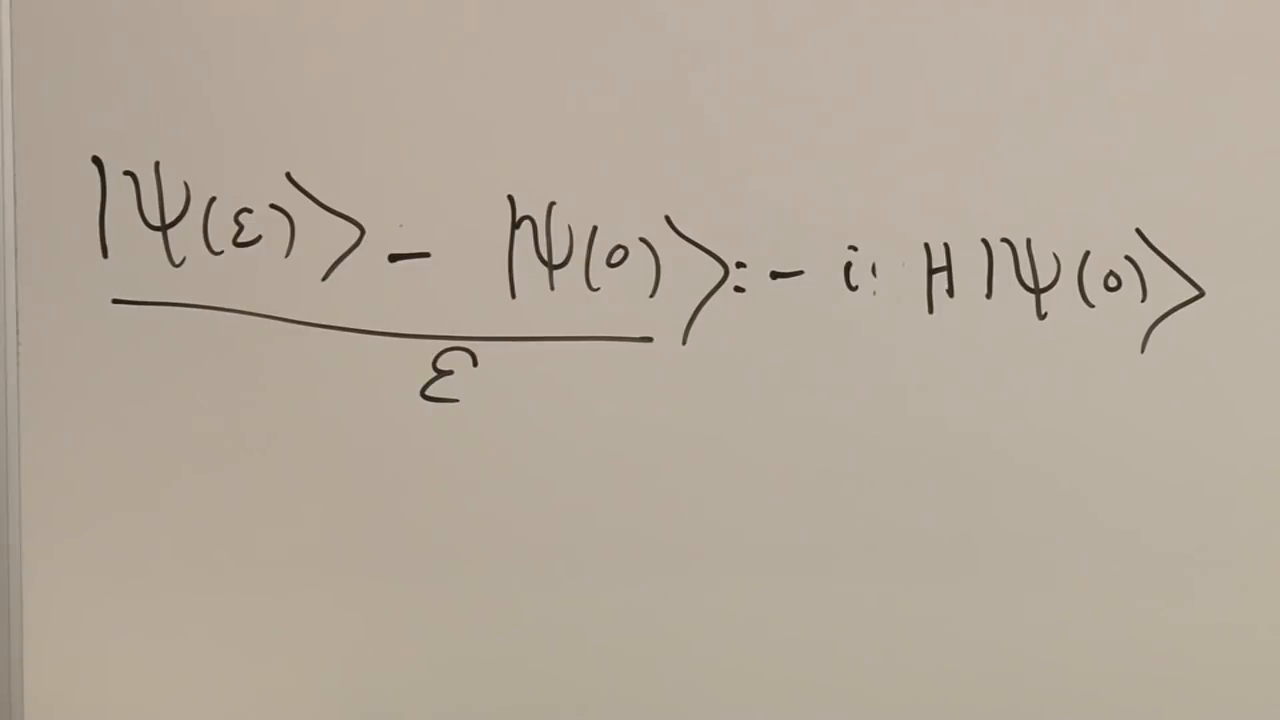
\includegraphics[width=0.86\textwidth]{lecture_05_figure_03.png}
\caption{Cập nhật vô cùng bé được viết dưới dạng thương sai phân.}
\lectureframe{00:23:33}
\end{figure}

Lấy giới hạn \(\epsilon\to0\) cho ta phương trình Schr\"odinger phụ thuộc thời gian:
\begin{equation}
\frac{d}{dt}\ket{\psi(t)}=-iH\ket{\psi(t)}.
\label{eq:l5-schrodinger}
\end{equation}
Khôi phục các hằng số, ta có \(i\hbar\,d\ket{\psi}/dt=H\ket{\psi}\).

Phương trình ban đầu của Schr\"odinger nói về hàm sóng của một hạt chuyển động. Phát biểu ở dạng toán tử ở trên từng được gọi là phương trình Schr\"odinger tổng quát hóa vì nó áp dụng như nhau cho một spin, một hệ ba trạng thái, hai spin, hay một hệ có độ phức tạp tùy ý. Tính từ đó phần lớn đã bị lược bỏ; hiện nay đây đơn giản là dạng tổng quát của phương trình ấy.

Phương trình~\eqref{eq:l5-schrodinger} cho sự tiến hóa xác định của trạng thái khi hệ được để yên không bị nhiễu. Điều đó không làm cho mọi kết quả thực nghiệm đều xác định. Một trạng thái lượng tử xác định các xác suất cho những phép đo có thể xảy ra, và phương trình cập nhật các xác suất đó thông qua các biên độ đang thay đổi. Phép đo nói chung làm thay đổi trạng thái và làm gián đoạn sự tiến hóa cô lập này.

\begin{classroomqa}
\audiencequestion{Mọi phép đo đều làm nhiễu hệ sao?}
\lecturerresponse{Nói chung là có, nhưng có một trường hợp đặc biệt quan trọng. Nếu trạng thái đã là một trạng thái riêng của đại lượng quan sát, thì một phép đo lý tưởng có thể lặp lại được có thể xác nhận giá trị của nó mà không làm thay đổi trạng thái ấy. Điều nói chung không thể làm được là đo một đại lượng quan sát tùy ý mà không làm nhiễu các tính chất khác, không tương thích.}
\end{classroomqa}

\section{Năng lượng và phương trình không phụ thuộc thời gian}

Vì \(H\) là Hermite, các trị riêng của nó là thực và các vectơ riêng của nó có thể được chọn thành một cơ sở trực chuẩn đầy đủ:
\begin{equation}
H\ket{E_i}=E_i\ket{E_i}.
\label{eq:l5-time-independent}
\end{equation}
Đây là dạng không phụ thuộc thời gian của phương trình Schr\"odinger. Nó là một bài toán trị riêng chứ không phải một phương trình chuyển động: nó hỏi hệ có thể có những giá trị năng lượng nào và những trạng thái nào có các giá trị ấy một cách sắc nét.

Phổ phụ thuộc vào hệ. Chuyển động nguyên tử liên kết và dao động tử điều hòa có các mức năng lượng đếm được. Một hạt không liên kết có thể có phổ liên tục. Năng lượng có thể được đo theo nhiều cách; về nguyên tắc, ngay cả một phép đo khối lượng đủ chính xác cũng có thể dùng \(E=mc^2\), mặc dù đó hiếm khi là phương pháp thực hành. Một hệ thực đã có sẵn Hamiltonian của nó; nhà vật lý không áp đặt nó mà cố gắng khám phá nó. Một khi toán tử đó đã biết, việc tìm các trị riêng và vectơ riêng của nó là nhiệm vụ toán học.

Cộng một hằng số \(cI\) vào \(H\) sẽ dịch mọi năng lượng thêm \(c\). Nó nhân toàn bộ trạng thái với một pha chung duy nhất \(e^{-ict}\), điều này không làm thay đổi xác suất hay giá trị kỳ vọng. Chỉ các độ chênh năng lượng mới ảnh hưởng đến động lực học được xét ở đây.

\section{Giá trị kỳ vọng biến đổi như thế nào}

Cụm từ chuẩn \emph{giá trị kỳ vọng} có nghĩa là một trung bình thống kê. Với một đại lượng quan sát \(L\),
\begin{equation}
\expect{L}(t)=\bra{\psi(t)}L\ket{\psi(t)}.
\end{equation}
Ở giai đoạn này, chỉ các vectơ trạng thái mang sự phụ thuộc theo thời gian. Lấy đạo hàm hai vế và dùng Phương trình~\eqref{eq:l5-schrodinger} cùng với liên hợp Hermite của nó,
\begin{equation}
\frac{d}{dt}\ket{\psi}=-iH\ket{\psi},
\qquad
\frac{d}{dt}\bra{\psi}=i\bra{\psi}H,
\end{equation}
ta được
\begin{align}
\frac{d}{dt}\expect{L}
&=i\bra{\psi}HL\ket{\psi}
  -i\bra{\psi}LH\ket{\psi}\\
&=-i\expect{[L,H]}.
\label{eq:l5-expectation-motion}
\end{align}

\begin{figure}[htbp]
\centering
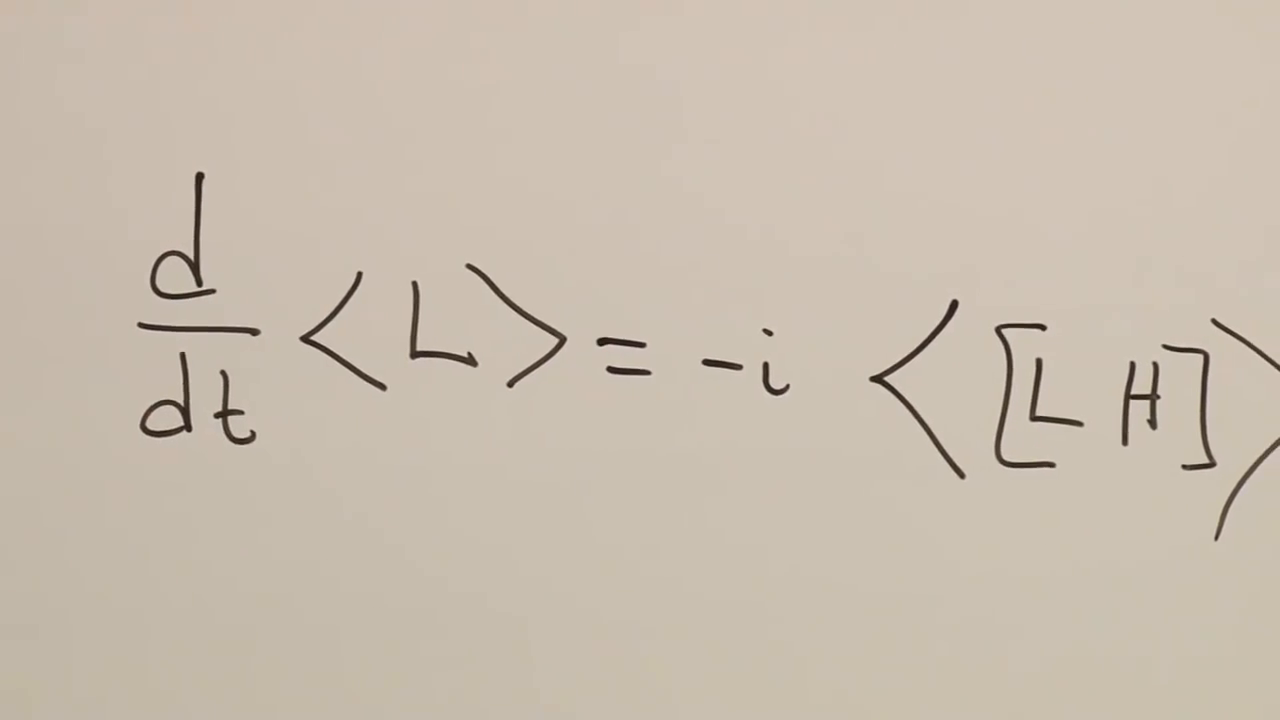
\includegraphics[width=0.86\textwidth]{lecture_05_figure_04.png}
\caption{Phương trình chuyển động của giá trị kỳ vọng dưới dạng giao hoán tử.}
\lectureframe{00:35:35}
\end{figure}

Thừa số \(i\) không đe dọa tính thực của \(\expect{L}\). Với \(L\) và \(H\) là Hermite, giao hoán tử là phản-Hermite:
\begin{equation}
[L,H]^\dagger=-[L,H].
\end{equation}
Vì thế giá trị kỳ vọng của nó là thuần ảo, nên nhân với \(-i\) sẽ cho một đạo hàm thực.

Đôi khi người ta viết dạng rút gọn
\begin{equation}
\dot L=-i[L,H].
\end{equation}
Ở thời điểm này, nó nên được hiểu là cách viết tắt của Phương trình~\eqref{eq:l5-expectation-motion}, tức một phương trình về các giá trị trung bình. Việc đổi hẳn sang một biểu diễn trong đó bản thân các toán tử mang sự phụ thuộc theo thời gian sẽ được trình bày sau.

\subsection{Đại số của các giao hoán tử}

Các giao hoán tử là phản đối xứng:
\begin{equation}
[A,B]=-[B,A].
\end{equation}
Chúng cũng tuân theo một quy tắc tích tương tự quy tắc Leibniz cho đạo hàm:
\begin{equation}
[AB,C]=A[B,C]+[A,C]B.
\label{eq:l5-product-rule}
\end{equation}
Để kiểm tra điều đó, hãy giữ nguyên thứ tự của mọi thừa số:
\begin{align}
A[B,C]+[A,C]B
&=A(BC-CB)\\
&\quad +(AC-CA)B\\
&=ABC-ACB\\
&\quad +ACB-CAB\\
&=ABC-CAB\\
&=[AB,C].
\end{align}

\begin{figure}[htbp]
\centering
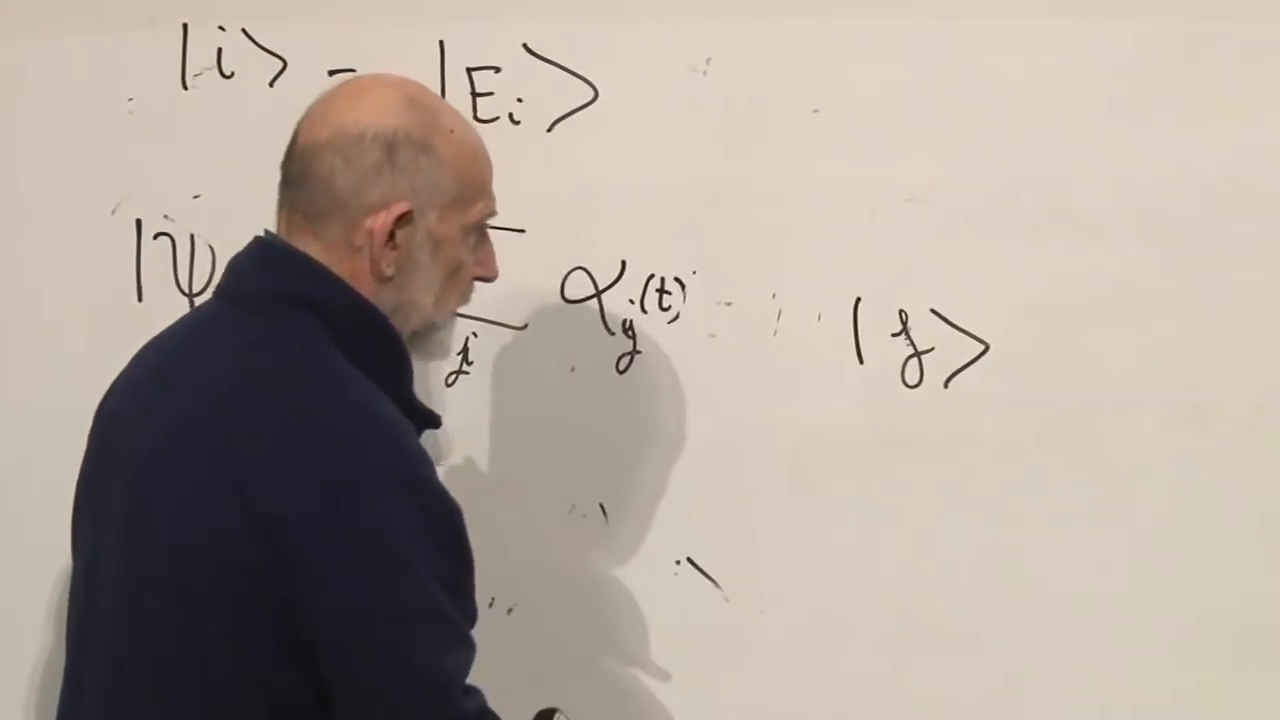
\includegraphics[width=0.86\textwidth]{lecture_05_figure_05.png}
\caption{Quy tắc tích của giao hoán tử được kiểm tra bằng cách khai triển cả hai vế.}
\lectureframe{00:43:10}
\end{figure}

\begin{classroomqa}
\audiencequestion{Vế phải của quy tắc tích có vô tình đếm vế trái hai lần không?}
\lecturerresponse{Không. Khi khai triển, \(ABC\) và \(-CAB\) là hai hạng tử mong muốn. Hai hạng tử được chèn vào là \(-ACB\) và \(+ACB\), chúng triệt tiêu nhau chính xác. Bản sao có vẻ thừa ấy là hạng tử tạm thời cần để phân tích biểu thức theo hai cách cần thiết.}
\end{classroomqa}

Cùng tính phản đối xứng và quy tắc tích ấy cũng đúng cho các ngoặc Poisson cổ điển. Sự giống nhau về cấu trúc này không phải là ngẫu nhiên. Phép tương ứng cổ điển là
\begin{equation}
\{A,B\}
\quad\longleftrightarrow\quad
\frac{1}{i\hbar}[A,B]
=-\frac{i}{\hbar}[A,B].
\label{eq:l5-poisson-correspondence}
\end{equation}
Trong đơn vị \(\hbar=1\), phương trình cổ điển
\begin{equation}
\frac{dL}{dt}=\{L,H\}
\end{equation}
có cùng dạng với Phương trình~\eqref{eq:l5-expectation-motion}. Trong các đơn vị thông thường ở thang vĩ mô, \(\hbar\) rất nhỏ, và các giao hoán tử trở nên không đáng kể trong giới hạn cổ điển thích hợp. Đây là phép kiểm tra cốt yếu để đồng nhất bộ sinh lượng tử \(H\) với Hamiltonian của cơ học cổ điển.

Thừa số \(\hbar\) là cần thiết về mặt thứ nguyên. Một ngoặc Poisson lấy đạo hàm theo các tọa độ và xung lượng liên hợp, trong khi một giao hoán tử toán tử được xây dựng trực tiếp từ các tích. Hằng số Planck cung cấp phép chuyển đổi giữa các thứ nguyên đó.

Đặt \(L=H\). Vì mọi toán tử đều giao hoán với chính nó,
\begin{equation}
\frac{d}{dt}\expect{H}
=-i\expect{[H,H]}=0.
\end{equation}
Đối với các Hamiltonian không phụ thuộc thời gian đang bàn ở đây, năng lượng trung bình được bảo toàn. Có thể đưa ra một phát biểu mạnh hơn về toàn bộ phân bố năng lượng, nhưng ở đây giá trị trung bình là tất cả những gì cần đến.

\begin{classroomqa}
\audiencequestion{Trong các phương trình này, \(L\) là gì? Có phải mômen góc không?}
\lecturerresponse{Ở đây \(L\) là một toán tử tuyến tính Hermite tổng quát, nên là một đại lượng quan sát bất kỳ. Nó có thể là một thành phần spin, một vị trí, hay thậm chí chính \(H\). Chữ cái này được chọn cho \emph{toán tử tuyến tính} và không nên được hiểu là mômen góc trừ khi ý nghĩa đó được nêu riêng.}
\end{classroomqa}

\begin{classroomqa}
\audiencequestion{Tại sao thừa số \(i\) không làm cho một giá trị kỳ vọng thực có đạo hàm ảo?}
\lecturerresponse{Giao hoán tử của hai toán tử Hermite là phản-Hermite, nên giá trị kỳ vọng của nó là ảo. Phép tính với các ma trận Pauli ở dưới làm điều này trở nên cụ thể: các giao hoán tử của chúng chứa một thừa số hiện tường minh \(2i\), thừa số này triệt tiêu \(-i\) trong phương trình chuyển động.}
\end{classroomqa}

\section{Giải phương trình Schr\"odinger trong cơ sở năng lượng}

Giả sử bài toán trị riêng năng lượng đã được giải. Khai triển một trạng thái bất kỳ theo cơ sở năng lượng cố định:
\begin{equation}
\ket{\psi(t)}=\sum_j\alpha_j(t)\ket{E_j}.
\label{eq:l5-energy-expansion}
\end{equation}
Trong mô tả này, các vectơ cơ sở không thay đổi; toàn bộ sự phụ thuộc thời gian nằm trong các hệ số. Thế Phương trình~\eqref{eq:l5-energy-expansion} vào Phương trình~\eqref{eq:l5-schrodinger} thu được
\begin{align}
\sum_j\dot\alpha_j(t)\ket{E_j}
&=-i\sum_j\alpha_j(t)H\ket{E_j}\\
&=-i\sum_j E_j\alpha_j(t)\ket{E_j}.
\end{align}
Tính duy nhất của khai triển theo một cơ sở kéo theo rằng, với mỗi \(j\) cố định,
\begin{equation}
\dot\alpha_j(t)=-iE_j\alpha_j(t),
\qquad\text{no sum on \(j\)}.
\end{equation}
Nghiệm là
\begin{equation}
\alpha_j(t)=\alpha_j(0)e^{-iE_jt}.
\label{eq:l5-energy-phase}
\end{equation}

\begin{figure}[htbp]
\centering
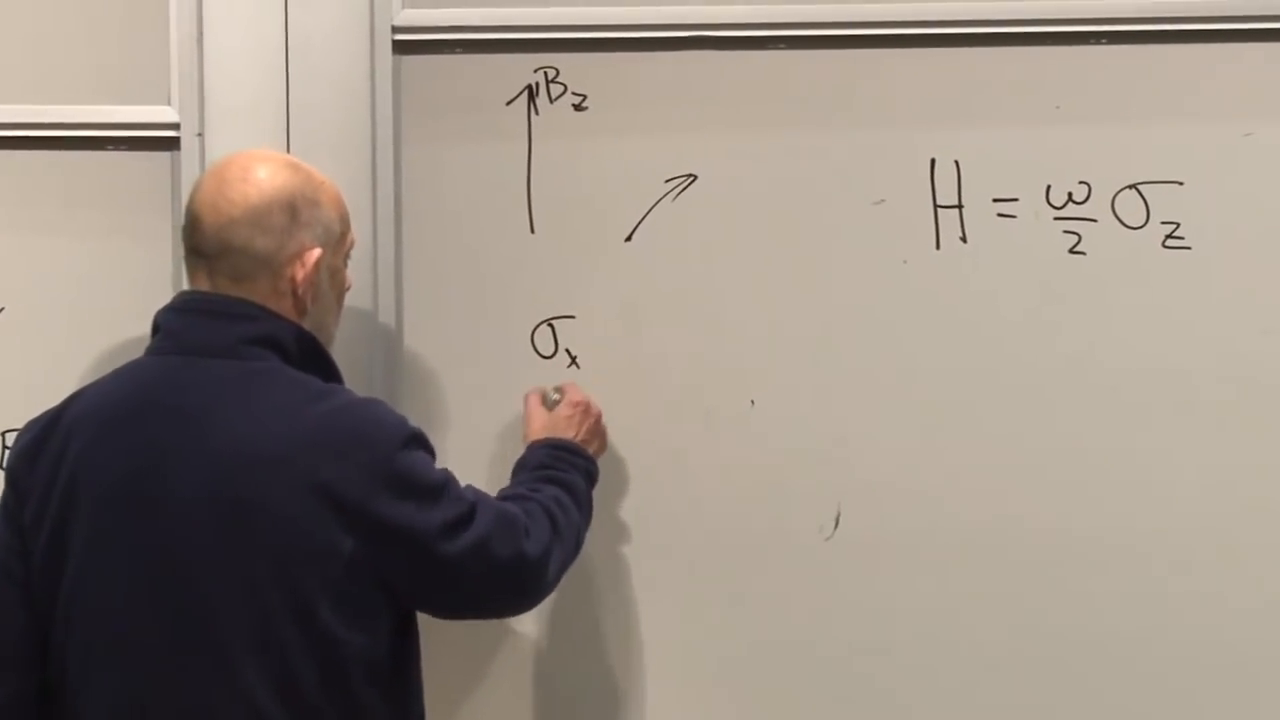
\includegraphics[width=0.86\textwidth]{lecture_05_figure_06.png}
\caption{Mỗi hệ số trong cơ sở năng lượng thỏa mãn phương trình pha dạng hàm mũ riêng.}
\lectureframe{01:03:25}
\end{figure}

Vì vậy nghiệm tổng quát là
\begin{equation}
\ket{\psi(t)}
=\sum_j\alpha_j(0)e^{-iE_jt}\ket{E_j}.
\label{eq:l5-general-solution}
\end{equation}
Khôi phục đơn vị sẽ thay \(E_jt\) bằng \(E_jt/\hbar\). Độ lớn của mỗi hệ số giữ nguyên:
\begin{equation}
|\alpha_j(t)|=|\alpha_j(0)|.
\end{equation}
Sự tiến triển theo thời gian làm thay đổi các pha tương đối. Một trạng thái riêng năng lượng đơn lẻ chỉ nhận một pha chung duy nhất và do đó có các xác suất đo độc lập với thời gian.

Giờ đây có thể viết tường minh giá trị kỳ vọng của \(L\). Định nghĩa các phần tử ma trận của nó trong cơ sở năng lượng bởi
\begin{equation}
L_{kj}=\bra{E_k}L\ket{E_j}.
\end{equation}
Khi đó
\begin{align}
\expect{L}(t)
&=\sum_{k,j}
\alpha_k^*(0)\alpha_j(0)
e^{i(E_k-E_j)t}
L_{kj}.
\label{eq:l5-heisenberg-matrix}
\end{align}

\begin{figure}[htbp]
\centering
\includegraphics[width=0.86\textwidth]{lecture_05_figure_07.png}
\caption{Công thức ma trận trong cơ sở năng lượng: mỗi phần tử mang một pha ứng với tần số chuyển tiếp.}
\lectureframe{01:10:45}
\end{figure}

Các hạng chéo \(k=j\) là hằng. Một phần tử ma trận ngoài đường chéo dao động với hiệu năng lượng \(E_k-E_j\). Theo tường thuật lịch sử được nêu ở đây, Heisenberg đã nhận ra cách tổ chức ma trận này trước khi phép suy ra hiện đại bằng vectơ trạng thái xuất hiện; về sau ký hiệu của Dirac làm cho ý nghĩa của nó trở nên minh bạch.

\begin{classroomqa}
\audiencequestion{Độ lớn của các hệ số \(\alpha_j\) có giữ nguyên không?}
\lecturerresponse{Có. Mỗi hệ số được nhân với một pha phức có độ lớn đơn vị. Chỉ các pha tương đối thay đổi, và chính các pha đó cho phép các giá trị kỳ vọng có chứa các phần tử ma trận ngoài đường chéo biến thiên theo thời gian.}
\end{classroomqa}

\begin{classroomqa}
\audiencequestion{Phương trình Schr\"odinger nên dùng đạo hàm riêng hay đạo hàm toàn phần?}
\lecturerresponse{Đối với trạng thái trừu tượng \(\ket{\psi(t)}\) được dùng ở đây, thời gian là biến duy nhất được hiển thị, nên ký hiệu nào cũng mang cùng một nội dung. Về sau một hàm sóng như \(\psi(x,t)\) sẽ phụ thuộc cả vị trí lẫn thời gian, và khi đó ký hiệu đạo hàm riêng sẽ là tự nhiên.}
\end{classroomqa}

\begin{classroomqa}
\audiencequestion{Việc bảo toàn tính trực giao có chỉ đơn thuần là một giả định thực nghiệm không?}
\lecturerresponse{Nó được thực nghiệm ủng hộ, nhưng đồng thời cũng cứng nhắc một cách khác thường. Những nỗ lực làm biến dạng cơ học lượng tử unita có xu hướng phá hủy tính dương hoặc sự bảo toàn xác suất, tính địa phương nhân quả, hoặc cách xử lý nhất quán các hệ hợp thành. David Finkelstein mô tả các lý thuyết có thể biến dạng như trải qua chảy dẻo và các lý thuyết cứng như nứt gãy giòn. Cơ học lượng tử là giòn theo nghĩa này: những thay đổi tùy ý nhỏ thường không để lại một lý thuyết nhất quán lân cận.}
\end{classroomqa}

\begin{classroomqa}
\audiencequestion{Vì sao các trị riêng năng lượng \(E_j\) là thực?}
\lecturerresponse{Tính unita hàm ý rằng bộ sinh vô cùng bé \(H\) là Hermite, và mọi trị riêng của một toán tử Hermite đều là số thực. Vì vậy chuỗi suy luận là: bảo toàn tính trực giao, tính unita, tính Hermite của \(H\), và tính thực của phổ năng lượng.}
\end{classroomqa}

\section{Một spin trong từ trường}

Nên gán Hamiltonian nào cho một spin? Một spin cô lập trong không gian ngoài ra trống rỗng không có phương ưu tiên không tầm thường nào, nên Hamiltonian của nó tỉ lệ với toán tử đơn vị và không tạo ra chuyển động quan sát được. Một từ trường cung cấp cả năng lượng tương tác lẫn một trục.

Lấy từ trường dọc theo \(z\). Một hạt mang điện có spin mang một mômen từ, và năng lượng lưỡng cực quen thuộc tỉ lệ với sự thẳng hàng của mômen đó với trường. Gộp độ mạnh của trường, mômen từ, quy ước dấu và \(\hbar\) vào một hằng số \(\omega\):
\begin{equation}
H=\frac{\omega}{2}\sigma_z.
\label{eq:l5-z-hamiltonian}
\end{equation}
Thừa số \(1/2\) thuận tiện vì các giao hoán tử Pauli chứa một thừa số \(2\).

Hình dung mũi tên cổ điển phải được xử lý cẩn thận. Một spin lượng tử không đồng thời có các thành phần \(x\), \(y\) và \(z\) xác định, nên không một mũi tên thông thường nào có thể biểu diễn mọi tính chất của nó cùng một lúc. Đối tượng ba chiều hữu ích sẽ là vectơ các giá trị kỳ vọng, chứ không phải chính vectơ trạng thái hai thành phần.

\subsection{Các giao hoán tử Pauli}

Dùng các biểu diễn ma trận
\begin{equation}
\begin{aligned}
\sigma_x&=
\begin{pmatrix}0&1\\1&0\end{pmatrix},\\[0.4em]
\sigma_y&=
\begin{pmatrix}0&-i\\i&0\end{pmatrix},\\[0.4em]
\sigma_z&=
\begin{pmatrix}1&0\\0&-1\end{pmatrix}.
\end{aligned}
\end{equation}
Ví dụ,
\begin{align}
[\sigma_z,\sigma_x]
&=
\begin{pmatrix}1&0\\0&-1\end{pmatrix}
\begin{pmatrix}0&1\\1&0\end{pmatrix}
-
\begin{pmatrix}0&1\\1&0\end{pmatrix}
\begin{pmatrix}1&0\\0&-1\end{pmatrix}\\
&=
\begin{pmatrix}0&1\\-1&0\end{pmatrix}
-
\begin{pmatrix}0&-1\\1&0\end{pmatrix}\\
&=2
\begin{pmatrix}0&1\\-1&0\end{pmatrix}
=2i\sigma_y.
\end{align}
Các hệ thức chu kỳ là
\begin{equation}
\begin{aligned}
[\sigma_z,\sigma_x]&=2i\sigma_y,\\
[\sigma_x,\sigma_y]&=2i\sigma_z,\\
[\sigma_y,\sigma_z]&=2i\sigma_x.
\end{aligned}
\label{eq:l5-pauli-commutators}
\end{equation}
Đảo thứ tự của một trong hai toán hạng thì đổi dấu.

\begin{figure}[htbp]
\centering
\includegraphics[width=0.86\textwidth]{lecture_05_figure_08.png}
\caption{Ba giao hoán tử Pauli khép kín theo chu kỳ trên chính các ma trận Pauli.}
\lectureframe{01:33:30}
\end{figure}

Các hệ thức này có cùng cấu trúc chu kỳ như các ngoặc Poisson cổ điển của mômen động lượng. Chúng cũng khép kín trên chính ba toán tử ban đầu, điều này làm cho các phương trình chuyển động đặc biệt đơn giản.

\begin{classroomqa}
\audiencequestion{Có bắt buộc phải tính các giao hoán tử bằng ký hiệu bra-ket không?}
\lecturerresponse{Không. Phép nhân toán tử được biểu diễn bằng phép nhân ma trận, nên các ma trận \(2\times2\) cung cấp một phép tính trực tiếp thuận tiện. Thay vào đó cũng có thể cho các toán tử tác dụng liên tiếp lên các trạng thái cơ sở lên và xuống và thu được cùng kết quả.}
\end{classroomqa}

\subsection{Sự tiến động của các giá trị kỳ vọng}

Áp dụng Phương trình~\eqref{eq:l5-expectation-motion} với Hamiltonian trong Phương trình~\eqref{eq:l5-z-hamiltonian}:
\begin{align}
\frac{d}{dt}\expect{\sigma_x}
&=-i\frac{\omega}{2}\expect{[\sigma_x,\sigma_z]}
=-\omega\expect{\sigma_y},\\
\frac{d}{dt}\expect{\sigma_y}
&=-i\frac{\omega}{2}\expect{[\sigma_y,\sigma_z]}
=+\omega\expect{\sigma_x},\\
\frac{d}{dt}\expect{\sigma_z}
&=-i\frac{\omega}{2}\expect{[\sigma_z,\sigma_z]}
=0.
\label{eq:l5-spin-motion}
\end{align}

\begin{figure}[htbp]
\centering
\begin{minipage}[c]{0.62\textwidth}
\centering
\includegraphics[width=\textwidth]{lecture_05_figure_09.png}
\end{minipage}\hfill
\begin{minipage}[c]{0.31\textwidth}
\centering
\begin{tikzpicture}[scale=0.78,>=Latex]
  \draw[->,thick] (0,0) -- (0,3.0) node[above] {\(z\parallel\bm B\)};
  \draw[dashed] (0,1.8) ellipse (1.45 and 0.42);
  \draw[->,very thick] (0,0) -- (1.05,1.8)
    node[right] {\(\expect{\bm\sigma}\)};
  \draw[->,thick] (1.38,1.67)
    arc[start angle=-12,end angle=245,x radius=1.45,y radius=0.42];
\end{tikzpicture}
\end{minipage}
\caption{Các phương trình trên bảng và hệ quả hình học của chúng: các giá trị trung bình vuông góc với trường quay tròn, còn thành phần song song với trường thì giữ nguyên. Mũi tên biểu diễn ba giá trị kỳ vọng, không phải một spin cổ điển ẩn.}
\lectureframe{01:35:28}
\end{figure}

Hai phương trình đầu mô tả chuyển động tròn trong mặt phẳng vuông góc với trường:
\begin{align}
\expect{\sigma_x}(t)
&=\expect{\sigma_x}(0)\cos\omega t
-\expect{\sigma_y}(0)\sin\omega t,\\
\expect{\sigma_y}(t)
&=\expect{\sigma_x}(0)\sin\omega t
+\expect{\sigma_y}(0)\cos\omega t.
\end{align}
Trong khi đó \(\expect{\sigma_z}\) là hằng. Do đó vectơ giá trị kỳ vọng tiến động quanh trục từ trường với tần số góc \(\omega\).

Trong phép tính ở biểu diễn Schr\"odinger này, các toán tử là những ma trận cố định. Chính trạng thái thay đổi, và vì thế các giá trị kỳ vọng thực hiện chuyển động con quay quen thuộc.

\begin{classroomqa}
\audiencequestion{Làm sao một không gian trạng thái hai chiều lại có thể cho ra một hình ảnh tiến động ba chiều?}
\lecturerresponse{Vectơ trạng thái có hai thành phần phức, nếu bỏ qua chuẩn hóa và pha tổng thể. Ngược lại, vectơ trong không gian thực được vẽ ra là \(\bigl(\expect{\sigma_x},\expect{\sigma_y},\expect{\sigma_z}\bigr)\). Các giá trị kỳ vọng này được xác định bởi trạng thái và tạo thành hình ảnh vectơ Bloch, nhưng chúng không phải chính vectơ trạng thái.}
\end{classroomqa}

\section{Hamiltonian tổng quát nhất của một spin}

Mọi ma trận Hermite \(2\times2\) đều có thể khai triển thành
\begin{equation}
H=aI+b_x\sigma_x+b_y\sigma_y+b_z\sigma_z,
\end{equation}
với các hệ số thực. Hạng đơn vị chỉ làm thay đổi pha tổng thể. Ba hệ số còn lại có thể được xem như các thành phần của một vectơ. Viết độ lớn của chúng là \(\omega/2\) và hướng của chúng là một vectơ đơn vị \(\bm n\), Hamiltonian không tầm thường trở thành
\begin{equation}
H=\frac{\omega}{2}\,\bm\sigma\cdot\bm n,
\qquad
\bm\sigma\cdot\bm n
=n_x\sigma_x+n_y\sigma_y+n_z\sigma_z.
\label{eq:l5-general-spin-h}
\end{equation}
Nếu \(\bm B=B\bm n\), thì \(\bm n\) mang hướng của trường còn \(\omega\) mang độ lớn của nó cùng với độ ghép từ. Chính \(\bm n\), chứ không phải \(\omega\), mới mã hóa định hướng.

Phương trình chuyển động có dạng gọn
\begin{equation}
\frac{d}{dt}\expect{\bm\sigma}
=\omega\,\bm n\times\expect{\bm\sigma}.
\end{equation}
Thành phần dọc theo \(\bm n\) giao hoán với \(H\) và giữ nguyên; các thành phần vuông góc tiến động quanh \(\bm n\).

\begin{classroomqa}
\audiencequestion{Vì sao đây là dạng đúng của Hamiltonian?}
\lecturerresponse{Chỉ có bốn ma trận Hermite độc lập \(2\times2\): \(I,\sigma_x,\sigma_y,\sigma_z\). Hạng đơn vị không đóng góp chuyển động một-spin quan sát được, nên mọi Hamiltonian một-spin độc lập thời gian không tầm thường đều là một tổ hợp tuyến tính với hệ số thực của ba ma trận Pauli. Một từ trường gói ba hệ số đó thành một độ lớn và một hướng.}
\end{classroomqa}

\begin{classroomqa}
\audiencequestion{Chính xác thì \(\omega\) biểu diễn điều gì?}
\lecturerresponse{Đó là một vô hướng tỉ lệ với độ lớn của trường nhân với mômen từ, với các hằng số quy ước đã được hấp thụ vào trong nó. Nó ấn định cả tốc độ tiến động lẫn độ tách mức năng lượng. Vectơ đơn vị \(\bm n\) chỉ định hướng của trường.}
\end{classroomqa}

\subsection{Hai mức năng lượng}

Viết Phương trình~\eqref{eq:l5-general-spin-h} dưới dạng ma trận cho
\begin{equation}
\bm\sigma\cdot\bm n
=
\begin{pmatrix}
n_z & n_x-in_y\\
n_x+in_y & -n_z
\end{pmatrix}.
\end{equation}
Gọi các trị riêng của nó là \(\lambda_1,\lambda_2\). Vết của nó bằng không:
\begin{equation}
\lambda_1+\lambda_2=0.
\end{equation}
Với vectơ đơn vị \(n_x^2+n_y^2+n_z^2=1\), định thức của nó là
\begin{align}
\lambda_1\lambda_2
&=\det(\bm\sigma\cdot\bm n)\\
&=-n_z^2-(n_x-in_y)(n_x+in_y)\\
&=-(n_x^2+n_y^2+n_z^2)\\
&=-1.
\end{align}
Do đó hai trị riêng là
\begin{equation}
\lambda_\pm=\pm1.
\end{equation}

\begin{figure}[htbp]
\centering
\includegraphics[width=0.86\textwidth]{lecture_05_figure_10.png}
\caption{Vết và định thức xác định các trị riêng của \(\bm\sigma\cdot\bm n\) là \(+1\) và \(-1\).}
\lectureframe{01:59:20}
\end{figure}

Do đó,
\begin{equation}
E_\pm=\pm\frac{\omega}{2},
\qquad
\Delta E=E_+-E_-=\omega.
\label{eq:l5-spin-gap}
\end{equation}
Hướng của trường làm thay đổi các vectơ riêng năng lượng nhưng không làm thay đổi hai trị riêng này.

\begin{classroomqa}
\audiencequestion{Sự phát xạ photon liên quan thế nào tới các mức này?}
\lecturerresponse{Khi tính cả trường bức xạ, mức spin cao hơn có thể phân rã xuống mức thấp hơn bằng cách phát ra một photon có năng lượng \(\Delta E=\omega\) theo quy ước \(\hbar=1\) hiện tại. Khi đó spin lật giữa hai định hướng đối nhau dọc theo trục trường. Phép tính tiến động đã bỏ qua độ ghép bức xạ yếu này, nên một spin có thể tiến động nhiều lần trước khi phát xạ.}
\end{classroomqa}

\begin{classroomqa}
\audiencequestion{Vì sao từ trường được coi như một con số thay vì một toán tử lượng tử?}
\lecturerresponse{Nam châm tạm thời được xem như một thiết bị cổ điển nặng sao cho dao động và độ giật lùi của nó là không đáng kể. Một mô tả đầy đủ sẽ bao gồm nó trong một hệ lượng tử lớn hơn. Sự tách hệ-thiết bị mang tính thực dụng này được biện minh khi thiết bị có nhiều bậc tự do và các biến liên quan của nó dao động ít đến mức electron không thể làm thay đổi chúng một cách đáng kể.}
\end{classroomqa}

\begin{classroomqa}
\audiencequestion{Các phương trình tiến động trơn có mô tả từng phép thử riêng lẻ không?}
\lecturerresponse{Chúng mô tả các giá trị kỳ vọng, do đó là các giá trị trung bình trên những phép thử được chuẩn bị giống hệt nhau. Các phép đo riêng lẻ vẫn mang tính xác suất. Những mẫu lặp lại có xu hướng xấp xỉ giá trị trung bình lý thuyết, nhưng lý thuyết xác suất không bảo đảm một kết quả chính xác cho mọi dãy hữu hạn, cũng như một triệu lần tung đồng xu không nhất thiết phải có đúng một nửa là mặt ngửa.}
\end{classroomqa}

\begin{classroomqa}
\audiencequestion{Nếu spin hướng ngang, một chuyển mức có phát ra nửa photon không?}
\lecturerresponse{Không. Một trạng thái spin hướng ngang là chồng chập của hai trạng thái riêng năng lượng. Trong trường hợp đối xứng, nó có xác suất một nửa ở mức trên và một nửa ở mức dưới. Vì thế nó có thể phát ra một photon trọn vẹn có năng lượng \(\omega\), hoặc không phát gì cả. Năng lượng phát xạ trung bình của nó có thể là \(\omega/2\), nhưng không photon riêng lẻ nào mang một nửa độ tách mức.}
\end{classroomqa}

Đến đây chúng ta đã khảo sát hết động lực học độc lập thời gian không tầm thường của một spin đơn lẻ. Cùng một đại số từng báo hiệu tính bất định cũng tạo ra chuyển động của nó: các ma trận Pauli không giao hoán biến Hamiltonian thành sự tiến động, trong khi thành phần giao hoán với Hamiltonian vẫn được bảo toàn. Bước tăng độ phức tạp tiếp theo không phải là một Hamiltonian một-spin khác mà là một không gian trạng thái lớn hơn, nơi các hệ độc lập có thể được hợp thành và rối.
